\section{Relational and Non-Relational database models}
The Rational and Non-Relational database models are two different approaches for storing volumes of data in a datastore.
The Relational Database model is unique, and there is only one type of Relational Database \parencite{relational-vs-nosql-a-survey}, whereas NoSQL has multiple.
There are many different types of NoSQL databases, but only four models are commonly used: \emph{Document Databases, Key-value databases, Wide-column stores and Graph Databases} \parencite{mongodb-what-is-nosql}.



\subsection{What describes a relational database}
A relational database utilizes \emph{tables, columns, rows} and \emph{keys} to create structure and relationships \parencite{ibm-relational-databases}.
If you wish to store information about certain people into the database, the first step would be to create a table which contain the persons information as \emph{attributes} in the form of \emph{columns}.
Onces the \emph{columns} are defined, they may be populated with a persons data, so when a new persons' information is added to the table, a row is created based on the columns.\\

\begin{figure}[h]
    \centering
    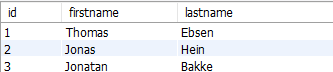
\includegraphics[scale=1.10]{/fig/relational-table.png}
    \caption{Figure of a Person Table in a relational database}
    \label{fig:relational-database-table}
\end{figure}

This makes visualization of the saved data easier for the user to understand. The implementation of a primary key is also a requirement when creating tables and it acts as a rows unique identifier. Figure~\ref{fig:relational-database-table} displays how a database table would look if the primary key is implemented as an auto incremented integer, however it can be defined by any value as long as it is unique \parencite{ibm-relational-databases}.
The primary key is crucial setting up relationships between tables, therefor it is important to choose the right unique identifier when defining it.

When creating tables, it is important to keep normalization in mind.
Database Normalization is a technique used to organize and structure the information in the database, in accordance to the so called 'normal-forms'. When applying normalization, a systematic approach is taken, to split the data into tables, as to prevent data redundancy and repetition \parencite{microsoft-normaliziation}.\\

An example of applying database normalization can be as followed:
\begin{figure}[h]
    \centering
    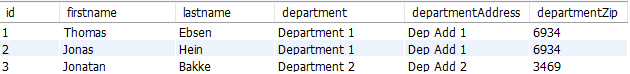
\includegraphics[scale=0.75]{/fig/relational-table-bad-normilazation.png}
    \caption{Figure of a Person Table in a relational database with no normalization}
    \label{fig:relational-database-table-normalization-bad}
\end{figure}

Figure~\ref{fig:relational-database-table-normalization-bad} display a databases table with no normalization, and by storing data this way, we quickly run into a data redundancy issue, where Thomas and Jonas' row contains some of the same data.
By applying normalization as we explained above, the updated database tables should be structured like this:
\begin{figure}[h]
    \centering
    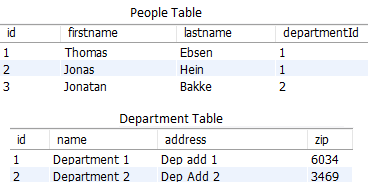
\includegraphics[scale=1.25]{/fig/relational-table-good-normilazation.png}
    \caption{Applying normalization to Fig~\ref{fig:relational-database-table-normalization-bad} to prevent redundancy}
    \label{fig:relational-database-table-normalization-good}
\end{figure}

This cleared the issue of reocurring information and reduced redundancy by making the department information reusable.

Aside from Normalization, which is not an actual requirement, ACID is.
All database that are built upon the Relational Database Model must adhere to the ACID principles. In layman's terms, ACID (Atomicity, Consistency, Isolation, Durability) references a set of standard properties that is used to guarantee that the database transactions are processed without issues \parencite{databaseguide-acid}.\\

As database.guide explains it, the different ACID properties do the following \parencite{databaseguide-acid}:
\begin{quotation}
    \emph{
    \noindent
    ``ACID is an acronym that stands for Atomicity, Consistency, Isolation, Durability. These are explained below.
    \begin{itemize}
        \item \textbf{Atomicity} means that you guarantee that either all of the transaction succeeds or none of it does. You don’t get part of it succeeding and part of it not. If one part of the transaction fails, the whole transaction fails. With atomicity, it’s either “all or nothing”.
        \item \textbf{Consistency} ensures that you guarantee that all data will be consistent. All data will be valid according to all defined rules, including any constraints, cascades, and triggers that have been applied on the database.
        \item \textbf{Isolation} Guarantees that all transactions will occur in isolation. No transaction will be affected by any other transaction. So a transaction cannot read data from any other transaction that has not yet completed.
        \item \textbf{Durability} means that, once a transaction is committed, it will remain in the system – even if there’s a system crash immediately following the transaction. Any changes from the transaction must be stored permanently. If the system tells the user that the transaction has succeeded, the transaction must have, in fact, succeeded.
    \end{itemize}
    }``
    - See https://database.guide \parencite{databaseguide-acid}
\end{quotation}

By complying with the ACID properties, the DBMS (Database Management System) ensures the organization who employs the relational database model database strategy, that their database will maintain data accuracy and consistency, even if a failure occurs during the transaction process \parencite{databaseguide-acid}.

\subsection{What describes a non-relational database}
\label{sec:what-describes-a-non-relational-database}
A Non-Relational database which is also called NoSQL or "not only SQL" \parencite{mongodb-what-is-nosql}, is a type of database that does not use the tabular form to store its data, but instead uses different data models, like the Document Database Model which we will use as a baseline for this section.
In the Document Database Model, the storing of data differ from the standard tabular structure, in the way that it can store different types of data inside a document without validating the data, which means it is essentially possible to store any type of data into a document \parencite{mongodb-non-relational-database}.
This type of storage method, is what makes it possible to store large and unstructured volumes of data easily, which means it is also much easier to import data sheets directly into the document, as it's setup is based on the data it received.

If you were to have an extensive CSV file filled with different information, that you wish to add into your database, it would prove difficult to do with traditional relational databases, since you would need to create tables for each different object in the csv and generate unique identifiers.
With NoSQL, the task is relatively straight forward, since it's not bound by relational restrictions. By using NoSQL's document based model, we can save the CSV file directly into the database without any prior processing by the help of mongoimport \parencite{databaseguide-mongo-csv}. The command will automatically convert it into a document, take the headers from the csv and convert them into value pairs and then save the data accordingly.